% Options for packages loaded elsewhere
\PassOptionsToPackage{unicode}{hyperref}
\PassOptionsToPackage{hyphens}{url}
%
\documentclass[
  12pt,
  openany]{book}
\usepackage{lmodern}
\usepackage{setspace}
\usepackage{amsmath}
\usepackage{ifxetex,ifluatex}
\ifnum 0\ifxetex 1\fi\ifluatex 1\fi=0 % if pdftex
  \usepackage[T1]{fontenc}
  \usepackage[utf8]{inputenc}
  \usepackage{textcomp} % provide euro and other symbols
  \usepackage{amssymb}
\else % if luatex or xetex
  \usepackage{unicode-math}
  \defaultfontfeatures{Scale=MatchLowercase}
  \defaultfontfeatures[\rmfamily]{Ligatures=TeX,Scale=1}
\fi
% Use upquote if available, for straight quotes in verbatim environments
\IfFileExists{upquote.sty}{\usepackage{upquote}}{}
\IfFileExists{microtype.sty}{% use microtype if available
  \usepackage[]{microtype}
  \UseMicrotypeSet[protrusion]{basicmath} % disable protrusion for tt fonts
}{}
\makeatletter
\@ifundefined{KOMAClassName}{% if non-KOMA class
  \IfFileExists{parskip.sty}{%
    \usepackage{parskip}
  }{% else
    \setlength{\parindent}{0pt}
    \setlength{\parskip}{6pt plus 2pt minus 1pt}}
}{% if KOMA class
  \KOMAoptions{parskip=half}}
\makeatother
\usepackage{xcolor}
\IfFileExists{xurl.sty}{\usepackage{xurl}}{} % add URL line breaks if available
\IfFileExists{bookmark.sty}{\usepackage{bookmark}}{\usepackage{hyperref}}
\hypersetup{
  hidelinks,
  pdfcreator={LaTeX via pandoc}}
\urlstyle{same} % disable monospaced font for URLs
\usepackage[left=4cm, right=3cm, top=3cm, bottom=3cm]{geometry}
\usepackage{longtable,booktabs}
\usepackage{calc} % for calculating minipage widths
% Correct order of tables after \paragraph or \subparagraph
\usepackage{etoolbox}
\makeatletter
\patchcmd\longtable{\par}{\if@noskipsec\mbox{}\fi\par}{}{}
\makeatother
% Allow footnotes in longtable head/foot
\IfFileExists{footnotehyper.sty}{\usepackage{footnotehyper}}{\usepackage{footnote}}
\makesavenoteenv{longtable}
\usepackage{graphicx}
\makeatletter
\def\maxwidth{\ifdim\Gin@nat@width>\linewidth\linewidth\else\Gin@nat@width\fi}
\def\maxheight{\ifdim\Gin@nat@height>\textheight\textheight\else\Gin@nat@height\fi}
\makeatother
% Scale images if necessary, so that they will not overflow the page
% margins by default, and it is still possible to overwrite the defaults
% using explicit options in \includegraphics[width, height, ...]{}
\setkeys{Gin}{width=\maxwidth,height=\maxheight,keepaspectratio}
% Set default figure placement to htbp
\makeatletter
\def\fps@figure{htbp}
\makeatother
\setlength{\emergencystretch}{3em} % prevent overfull lines
\providecommand{\tightlist}{%
  \setlength{\itemsep}{0pt}\setlength{\parskip}{0pt}}
\setcounter{secnumdepth}{5}
\usepackage[none]{hyphenat}
\usepackage[cmyk]{xcolor} % Recommended by US-AB
\usepackage{lmodern} % Recommended by US-AB
\usepackage{fancyhdr}
\usepackage{etoolbox}
\patchcmd{\chapter}{\thispagestyle{plain}}{\thispagestyle{fancy}}{}{} % Removes plain pagestyle from chapter headings (otherwise, page numbers are centered)
\AtBeginDocument{\addtocontents{toc}{\protect\thispagestyle{empty}}} 
\pagestyle{empty} % This makes ToC without header/footer
\usepackage[skip=15pt]{caption} % This should increase space below captions (not tested)
\raggedbottom
\usepackage[noindentafter]{titlesec}
\usepackage{titlesec}
\titleformat{\chapter}{\normalfont\bfseries}{\thechapter.}{15pt}{}\titlespacing*{\chapter}{0pt}{-50pt}{0pt}
\titleformat{\section}{\normalfont\bfseries}{\thesection.}{1em}{}\titlespacing*{\section}{0pt}{0pt}{0pt}
\titleformat{\subsection}[runin]{\normalfont\bfseries}{\thesubsection.}{1em}{}

\usepackage{CJKutf8} % For Mandarin in Acknowledgments

% For guiding quote in beginning of intro:
\makeatletter
% \renewcommand{\@chapapp}{}% Not necessary...
\newenvironment{chapquote}[2][2em]
  {\setlength{\@tempdima}{#1}%
   \def\chapquote@author{#2}%
   \parshape 1 \@tempdima \dimexpr\textwidth-2\@tempdima\relax%
   \itshape}
  {\par\normalfont\hfill--\ \chapquote@author\hspace*{\@tempdima}\par\bigskip}
\makeatother
\usepackage{dvipsnames,svgnames,x11names}
\PassOptionsToPackage{dvipsnames,svgnames,x11names}{xcolor}
\usepackage{placeins}
\usepackage{titlesec}
\newcommand{\sectionbreak}{\clearpage}
\usepackage{amsmath}
\usepackage{wrapfig}
\usepackage{caption}
\captionsetup[figure]{font=scriptsize}
\usepackage{float}
\ifluatex
  \usepackage{selnolig}  % disable illegal ligatures
\fi
\newlength{\cslhangindent}
\setlength{\cslhangindent}{1.5em}
\newlength{\csllabelwidth}
\setlength{\csllabelwidth}{3em}
\newenvironment{CSLReferences}[2] % #1 hanging-ident, #2 entry spacing
 {% don't indent paragraphs
  \setlength{\parindent}{0pt}
  % turn on hanging indent if param 1 is 1
  \ifodd #1 \everypar{\setlength{\hangindent}{\cslhangindent}}\ignorespaces\fi
  % set entry spacing
  \ifnum #2 > 0
  \setlength{\parskip}{#2\baselineskip}
  \fi
 }%
 {}
\usepackage{calc}
\newcommand{\CSLBlock}[1]{#1\hfill\break}
\newcommand{\CSLLeftMargin}[1]{\parbox[t]{\csllabelwidth}{#1}}
\newcommand{\CSLRightInline}[1]{\parbox[t]{\linewidth - \csllabelwidth}{#1}\break}
\newcommand{\CSLIndent}[1]{\hspace{\cslhangindent}#1}

\author{}
\date{\vspace{-2.5em}}

\begin{document}

{
\setcounter{tocdepth}{3}
\tableofcontents
}
\setstretch{1.5}
\cleardoublepage
\pagestyle{fancy}
\fancyhf{}
\renewcommand{\headrulewidth}{0pt}
\fancyfoot[LE,RO]{\thepage}
\renewcommand{\floatpagefraction}{.9}

\setcounter{page}{9}

\hypertarget{abbreviations}{%
\chapter*{Abbreviations}\label{abbreviations}}
\addcontentsline{toc}{chapter}{Abbreviations}

\begin{tabular}{ll}
\toprule
Abbreviation & Term\\
\midrule
RPF & Ribosome Protected Fragment\\
TOP & Terminal oligopyrimidine\\
TE & Translation Efficiency\\
UTR & Untranslated region\\
uORF & upstream open reading frame\\
\bottomrule
\end{tabular}

\chapter{Introduction}

\section{Central dogma of gene expression}

Cells are constantly performing processes to ensure proper function or adapt to intracellular or extracellular stresses. This demands that proteins are changed in abundance to perform the neccessary task. The genetic code, or Deoxyribonucleic acid (DNA), is stored in the nucleus of a cell. This code stores the information of the amino acids sequence for each protein in the cell which dictates the initial shape, size and function of a protein.
The central dogma of molecular biology describes the path genetic information follows to become expressed as proteins. This gene expression pathway consists of multiple steps; DNA transcription, RNA- splicing, mRNA transport, mRNA storage, mRNA degradation, mRNA translation and protein degradation (\textbf{Figure \ref{fig:geneExprPath}}). Each step along the gene expression pathway can exert control thereby shaping protein expression.
Translational control (i.e.~regulation of mRNA translation) is the focus in this thesis.
As seen in \textbf{figure \ref{geneExprPath}}, mRNA translation dictates which mRNAs will be synthesized into proteins.

\begin{wrapfigure}{l}{0.6\textwidth}
  \includegraphics{./figures/GeneExprPath.pdf}
  \caption{**The gene expression pathway** - DNA is transcribed in pre-mRNA containing introns and exons. Via RNA-splicing different mRNA isoforms can be formed by splicing variations of intron / exon combination. The mature mRNA, consisting out ouf exons only, is then transported out of the cellular nucleus into the cytoplasm. mRNAs can follow multiple paths such as storage, degradation or transaltion. mRNAs are translated into proteins (i.e. protein synthesis), which in turn can ultimately be degraded. \label{fig:geneExprPath}}
\end{wrapfigure}

\section{mRNA translation}

For the vast majority of protein coding mRNAs,eukaryotic mRNA translation occurs in the cytoplasm, however a small subset of mRNAs is translated in the mitochondria. mRNA translation is a process that includes initiation, elongation, termination and ribosome recycling and is an essential process. \textbf{Figure \ref{fig:doodlemRNASteps}} gives a simple overview of these steps in succession. The next sections in these thesis will describe these processes in detail.

\begin{wrapfigure}{o}{1\textwidth}
  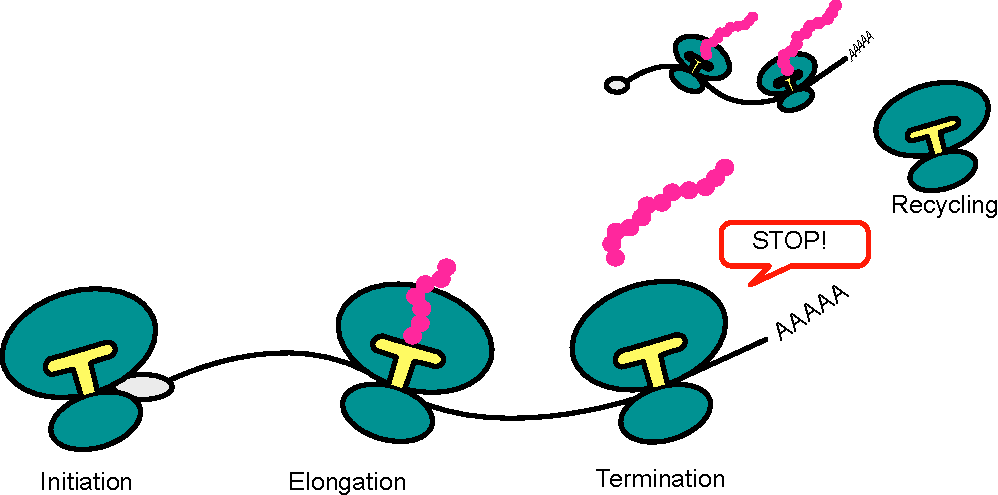
\includegraphics{./figures/doodleTranslation.pdf}
  \caption{**mRNA translation initiation, elongation, termination and ribosome recycling steps** - The ribosome binds to the mRNA and initiates scanning for a start codon. The elongation phase incorporates amino acids into a polypeptide chain (i.e. the protein product). Once the end of the coding sequence is detected, by recognition of stop codons, the ribosome terminates translation and releases the polypeptide chain. The ribosome can then be recycled to participate in the translation of another mRNA or reinitiate. \label{fig:doodlemRNASteps}}
\end{wrapfigure}
\clearpage
\subsection{mRNA translation initiation}

In eukaryotes most mRNAs are translated by scanning the mRNA for a start codon (AUG). This mechanism begins with the formation of the 43s pre-initiation complex (PIC) consisting of methionyl-initiator tRNA (met-tRNAi) in a ternary complex (TC) with guanosine triphosphate (GTP) bound eukaryotic initiation factor 2 (eIF2). The PIC is recruited to the 5'-cap of mRNAs which is facilitated by the eIF4F 5'-cap binding complex, a complex consisting of eIF4E (cap binding protein), eIF4A (RNA helicase) and eIF4G (scaffolding protein). The PIC then scans along the mRNA from the 5' end until it encounters an AUG codon. After AUG recognition eIF2-GTP is hydrolyzed forming a stable 48S PIC. Afterrelease of eIF2-GTP the 60S ribosomal subunit joins to form the 80S ribosome and protein synthesis can commenceDever \& Green (2012). Next to this scanning mechanism, mRNA translation can also be initiated via alternative cap independent mechanisms(Wurth \& Gebauer, 2015).

\subsection{mRNA translation elongation}

The 80S ribosome contains three sites; the acceptor (A), peptidyl (P) and Exit (E) sites. After initiation, the 80S ribosome is positioned with the met-tRNAi in the P site at the AUG codon with the following codon of the transcript in the A site awaiting its cognate tRNA. The tRNA arrives in a TC together with eukaryotic elongation factor 1A (eEF1A) at the A-site of the ribosome. After arrival in the A-site, the codon is then recognized. The binding of eEF1A is GTP dependent, recognition of the cognate codon by the tRNA triggers hydrolysis whereby eEF1A releases from the tRNA which is then recycled by eEF1B. Peptide bonds are then formed accompanied by a tRNA hybrid state whereby acceptor sites of tRNAs in the A-and P-site now move to the P-and E-site. Binding of eEF2-GTP then promotes translocation of the tRNAs into the P-and E-sites after which eEF2B-GDP releases. After release of the deacylated tRNA from the E-site the ribosome is ready for the next cycle. This process is repeated until a stop codon (UAA,UGA or UAG) is detected by the ribosome(Dever \& Green, 2012).

\subsection{mRNA translation termination}

is facilitated by two release factors, eRF2 and eRF3-GTP. The TC with eRF2 and eRF3-GTP binds to the A-site of the ribosome. Recognition of the stop codon by the ribosome then causes hydrolysis resulting in a conformational change and release of the polypeptide. eRF1 and the ATP binding cassette protein (ABCE1) together promote the splitting of the 60S and 40S subunits, of which the 40S subunits has still bound tRNA. After release of the tRNA from the 40S subunits the parts of the translational machinery can be recycled(Dever \& Green, 2012).

\section{Regulation of mRNA translation}

Of the heretofore presented steps of mRNA translation the initiation is the most regulated step. From the perspective that mRNA translation contributes most to the cellular energy consumption, of which the initiation requires ATP, this process ought to be strictly regulated Sonenberg \& Hinnebusch (2009). Nevertheless, translation can also be regulated at the elongation (Richter \& Coller, 2015) and termination(Dever \& Green, 2012) phases albeit to a lesser extent. Dynamic modulation of mRNA translation can be achieved through signalling pathways as well as several distinct cis and trans elements in both untranslated regions (UTRs) of an mRNA. mRNA translation can be regulated at a global level i.e.~reduction of protein synthesis for a large portion of the transcriptome. Furthermore, a more selective regulation of mRNA translation can be achieved through various mechanisms, which increases the complexity of the regulation of mRNA translation greatly.

\subsection{mTOR singalling pathway}

mTOR is a conserved Ser/Thr kinase and is found in two structurally and functionally distinct complexes, mTORC1 and mTORC2. mTORC1 contains mTOR, regulatory associated protein of TOR (raptor), the GTPase beta-subunit like protein (GbetaL) and disheveled, EGL-10, pleckstrin {[}DEP{]} domain containing mTOR-interacting protein (deptor). mLST8 and deptor are found in both mTORC1 and mTORC2.However, rapamycin-insensitive companion of TOR (rictor), mammalian stress-activated protein kinase {[}SAPK{]}-interacting protein (mSIN1), and proline-rich protein 5 (protor) are specific to mTORC2Pearce et al. (2007). In regards to regulation of mRNA translation, mTORC1 is a key player in regulation of translation initiation through facilitating the release of eIF4E from 4E-BPsvia phosphorylation of 4E-BPs by mTOR (Hsieh et al., 2010). Furthermore, substrates of mTORC1 include ribosomal S6 kinases (S6Ks) 1 and 2(Schepetilnikov et al., 2013), and La ribonucleoprotein domain family member 1 (LARP1)(Tcherkezian et al., 2014). mTORC2 is found to associate with ribosomes to promote co-translational phosphorylation and foldingofnascent Aktpolypeptide(Oh et al., 2010). As mentioned mTORC1 is activated via growth hormonesincludinginsulin and insulin like growth factor (IGF).For example,wheninsulin binds to the insulin receptor,tyrosine kinases (RTKs) and phosphoinositide 3-kinase (PI3K) are activated. Phosphatidylinositol 3,4,5-triphosphate (PIP3) is then generated by PI3K from Phosphatidylinositol 4,5-biphoasphate (PIP2). This step is reversed by PTEN which hydrolyzes PIP3 to PIP2, thereby working antagonistically to PI3K. PIP3 recruits AKT and phosphoinositide-dependent kinase1 (PDK1) towards the plasma membrane where AKT is phosphorylated by PDK1. Ras homologue enriched in brain (Rheb) is a GTPase that stimulates mTOR in its GTP bound form. The tuberous sclerosis complex (TSC) consists of TSC1 (scaffold protein) and TSC2 is a GTPase-activating protein (GAP) which inhibits Rheb through hydrolysis of Rheb-GTP to Rheb-GDP, thereby inhibiting mTOR activity. AKT mediates phosphorylation of TSC2, leading to a decreased GAP activity and reduced mTOR inhibition. Signaling through the Ras GTPase by growth factors may also activate mTORC1 through the RAF/MEK/ERK axis whereby extracellular signal-regulated kinase (ERK) leads to direct phosphorylation of TSC2 and raptor or via the RSKsLaplante \& Sabatini (2012).Protein synthesis is the most energy expensive process within cells(Buttgereit \& Brand, 1995).Therefore,regulation of mRNA translation is tied to cellular energy levels. AMP-activated protein kinase (AMPK) is a kinase activated by increased AMP/ATPratioas well as ADP/ATP ratios. AMPK inhibits protein synthesis by activation of TSC2, thereby reducing mTOR activity. Furthermore, cellular oxygen levels are linked to ATP production, where low oxygen levels reduce ATP production leading to AMPK activation(Leibovitch \& Topisirovic, 2018). mTOR modulates global mRNA translation mainly through modulation of 4E-BPs and S6KsHay \& Sonenberg (2004). S6Ks (S6K1 and S6K2) phosphorylates multiple component of the translational machinery such as RPS6, which is implicated in ribosome biogenesis(Magnuson, Ekim, \& Fingar, 2012). Furthermore, S6Ks also phosphorylates eEF2 kinase which is a negative regulator of protein synthesis(Wang et al., 2001).Lastly, S6Ks phosphorylate programmed cell death 4 (PDCD4)triggering its SCFbetaTrCP-dependent
degradation (Carayol et al., 2008).PDCD4 is a factor blocking the eIF4A-eIF4G interaction by binding to eIF4A. Binding of PDCD4 to eIF4A leads to inhibition of eIF4A activity and thus translation of mRNAs that require RNA helicase activity(Yang et al., 2003). More recent work has shown the interaction of mTORC1 with LA motif (LAM)-containing factor family La-related protein 1 (LARP1). LARP1 is thought to bind to the 5' mRNA cap of mRNAs with a terminal oloigopyrimidine motif (TOP) via its DM15 domain and represses translation thereof. Binding of LARP1 close the the 5' CAP of TOP mRNAs hinders binding of the EIF4F complex and therefore mRNA translation initiation. mTORC1 physically interacts and phosphorylates LARP1. When phophorylation occurs close to the DM15 domain of LARP1 the inhibitory effect on mRNA translation of TOP mRNAs is abolished. (Jia et al., 2021)

\subsection{The integrated stress response}

eIF2 delivers Met-tRNAi to the 40s ribosomal subunit (Sonenberg \& Hinnebusch, 2009). During the integrated stress response (ISR) the alpha subunit of eIF2 is phosphorylated on Ser51 which leads to a global suppression of 5' cap dependent mRNA translation. Upon eIF2alpha phosphorylation, eIF2alpha directly engages the guanine nucleotide exchange factor eIF2beta. eIF2beta converts the inactive eIF2-GDP to eIF2-GTP, therefore eIF2alpha phosphorylation limits eIF2 recycling of Met-tRNAi to the ribosome (Sonenberg \& Hinnebusch, 2009). Simultaneously, eIF2alpha phosphorylation stimulates selective translation of mRNAs with upstream open reading frames (uORFs) such as ATF4 which is a transcription factor that plays a crucial role in the adaptation to stress (Pakos-Zebrucka et al., 2016). There are multiple kinases, activated depending on the cellular stress, which phosphorylate eIF2alpha. These kinases include Protein kinase R-like endoplasmic reticulum kinase (PERK) which is activated by misfolded peptides in the endoplasmatic reticulum (ER), Heme regulated eIF2alpha kinase (HRI) which is activated during oxidative stress, protein kinase R (PKR) which is activated in response to certain viral infections and GCN2 which is activated when cells are deprived of amino acidsAndreev et al. (2015). Therefore, several distinct stress origins converge on the same pathway regulating mRNA translation.

\subsection{Regulation of translation through 5’ and 3’ UTRs}

is achieved via cis and trans elements.

Recruitment of the PIC to the 5' UTR is followed by scanning until recognition of a start codon. During scanning a process called leaky scanning can occur where the first encountered AUG is not recognized due to sub-optimal sequences flanking the start codon. Leaky scanning is influenced by eukaryotic elongation factors (eEF) 1 and eEF5 where high levels of eEF1 promote leaky scanning and blocking of non-cognate initiation whereas eEF5 works antagonistically to eEF1. Nonetheless, translation is most favorably initiated when an AUG is encountered with the ``Kozak'' context. Near cognate triplets e.g.~NUG can also initiate translation at a much lower frequency as compared to cognate triplets (Alan G. Hinnebusch, 2014). Structures in the 5' UTRs can influence translation initiation e.g.~stem loops (SL) like the iron responsive element (IRE), which regulates translation of mRNAs involved in iron homeostasis depending on iron availability (Paraskeva, Gray, Schläger, Wehr, \& Hentze, 1999) and RNA G-quadruplexes which block scanning (Wolfe et al., 2014). Therefore, the degree of structure of a 5' UTR can be an indicator whether an mRNA's translation efficiency is regulated or not. In eukaryotes the vast majority of mRNAs have 5' UTRs with a median length ranging from 53 to 218 nucleotides, where humans have 5' UTRs with the longest median length. Furthermore, mRNAs with long and structured 5' UTRs often encode for proteins related to proliferation, survival, and metastasis (Wolfe et al., 2014, p. Rubio2014).

Next to 5' UTR structures affecting cap dependent mRNA translation there are also cap independent regulators of mRNA translation such as the viral or cellular internal ribosome entry sites (IRES). The scope of the cellular IRES is still controversial, however cellular IRES are thought recruit the 43s ribosomal subunit towards the 5' UTR (Komar \& Hatzoglou, 2005). Additionally, eIF3 was suggested to directly bind to stem loop structures of a subset of mRNAs and repress or activate their translation Lee, Kranzusch, \& Cate (2015). RNA modifications in the 5' UTR could also potentially regulate mRNA translation such as the m6A modification, which can serve as an alternative cap and binds eIF3 to initiate translation or to assist ribosome scanning de la Parra et al. (2018).

Cis elements within the 5' UTR are also a found to regulate mRNA translation e.g.~mRNAs encoding for mitochondrial proteins with an extremely short (\textasciitilde12 nucleotides) 5' UTR which harbors the translation initiator of short 5' UTR (TISU element). These mRNAs undergo scanning free translation initiation (Haimov, Sinvani, \& Dikstein, 2015). Another well-studied 5' UTR element is the 5' terminal oligo pyrimidine (TOP) element, which consists of a C at the 5' terminus followed by a stretch of 4-15 pyrimidines (Yamashita et al., 2008). These TOP mRNAs are fully dependent on the C at the 5' cap. Translation of TOP mRNAs is tightly linked to mTOR activity and is often considered as mTOR dependent translation, where mTOR almost fully controls their translation activity (Hamilton, Stoneley, Spriggs, \& Bushell, 2006).

More recent work indicates an effect of mTORC1 on LA motif (LAM)-containing factor family La-related protein 1 (LARP1). In that study the conserved RNA-binding protein of LARP1 interacts with raptor and is phosphorylated by mTORC1. However, the scope of LARP1 mediated effects remain controversial. It has been suggested LARP1 stabilizes or regulates translation of mRNAs with the terminal oligo pyrimidine (TOP) motif in a context dependent manner{[}Tcherkezian et al. (2014),Bruno D. Fonseca et al. (2015),Deragon \& Bousquet-Antonelli (2015)).

Nevertheless, TOP mRNAs can contain other regulatory elements in their 5' UTR alongside the TOP motif, which can override the TOP element translational control in a context dependent manner (Avni, Biberman, \& Meyuhas, 1997).

The importance of the poly-A tail has been observed in several studies where the poly-A tail promotes efficient translation. mRNAs with short poly-A tails generally have a lower translational efficiency, however loss of a poly-A tail does not lead to complete inhibition of protein synthesis (Munroe \& Jacobson, 1990). Furthermore, there are many RNA- binding proteins binding to RNA elements in the 3' UTR such as PABP, CEBP and LARP1 which confer translational control Mendez \& Richter (2001). Cytoplasmic polyadenylation elements (CPEs) are U-rich sites in the 3' UTR (UUUUUAU) on which RNA binding proteins can bind (Mendez \& Richter, 2001). Cytoplasmic polyadenylation element binding proteins (CPEBs) are able to recruit either poly(A) polymerases e.g.~terminal nucleotidyltransferase 2 (TENT2) or deadenylation enzymes like the CCR4/NOT complex (Moore \& von Lindern, 2018). Therefore, the interaction of CPEBs with the recruited enzymes dictates whether a poly(A) tail is shortened or extended. Next to their predominant role in polyadenylation some members of the CPEB family are known to bind to general translation regulation factors, where CPEB4 binds eIF3 (Hu, Yuan, \& Lodish, 2014) and CPEB1 regulates mRNA stability by binding to PABPC1 and PABPC1L Guzeloglu-Kayisli et al. (2008). In Fragile X syndrome, an inheritable intelecutal disability, protein synthesis in the brain is elevated due to loss of FMRP. FMRP has been shown to be involved in ribosome stalling (Darnell et al., 2011) and therefore impacts ribosome elongation. An interesting interplay between FMRP and CEPB1 has been observed, where loss of both CEBP1 and FMRP could restore normal levels of protein synthesis (Udagawa et al., 2013). Poly-A-binding protein (PABP) is a multifunctional protein contributing to mRNA processing, stability and translation and is thought to bind to the 3' UTR. Regulation of translation by PABP is achieved through binding to various components of the translational machinery. These components include eIF4B, an initiation factor that aids RNA helicase unwinding function, and eIF4G , eukaryotic Release factor 3 (eRF3) which supports a role of PABP in ribosome recycling, and eIF3 Ivanov et al. (2016). Lastly, the PABP-eIF4G interaction forms the closed loop complex that connects the ends of the mRNA.

\subsection{Regulation of mRNA translation by tRNAs}

is a balance between supply and demand of charged tRNAs of actively translated codons. This concept is also referred to as codon optimality.

\subsection{Upstream open reading frames}

\section{Translation efficiency}

Each ribosome synthesises a single protein during translation of an mRNA from start to end. Typically an mRNA is loaded with multiple ribosomes (i.e.~polysomes). Therefore, the rate at which proteins can be synthesised is dependent on the availability of mRNAs as well as ribosome dynamics at the initiation, elongation and termination of mRNA translation.

\section{Regulatory modes of gene expression}

EXPAND EVOLUTION - NATURE PAPER COMENSATORY EFFECTS ETC
In transcriptome-wide studies of translation efficiencies the interplay between total mRNA and translated mRNA levels are interrogated. Traditionally it was thought that changes in translation efficiencies lead to altered protein levels. A change in translation efficiency is observed for mRNAs whose polysome-association is altered whereas their total mRNA does not change to a similar magnitude as the polysome-association (I.e. change in translation). An example thereof is TOP mRNA translation under conditions where mTOR is stimulated (Masvidal, Hulea, Furic, Topisirovic, \& Larsson, 2017).

\begin{wrapfigure}{l}{0.6\textwidth}
  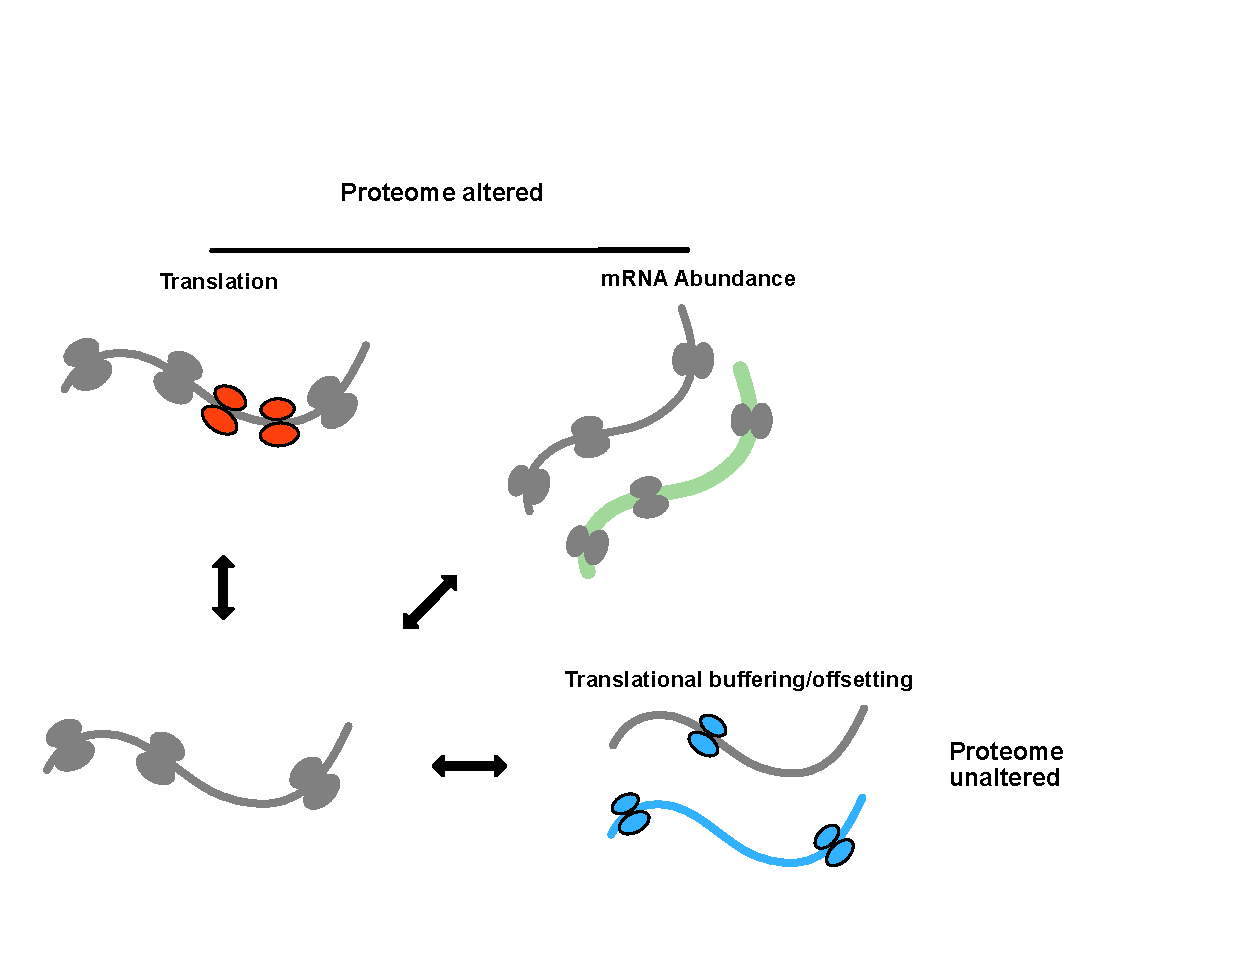
\includegraphics{./figures/geneModes_MRNA.pdf}
  \caption{Regulatory modes of gene expression - Schematic representation of regulatory modes of translation efficiency in a fold-change scatter plot. Indicated in red are changes in translation (i.e. changes in translated mRNA but not total mRNA), in green changes in mRNA abundance (i.e. congruent changes between total mRNA and translated mRNA) and in blue translational buffering (i.e. changes in total mRNA levels but not translated mRNA levels). TE changes as the TE-score would estimate them are indicated.\label{fig:mRNA}}
\end{wrapfigure}

In recent years, evidence emerged where translation efficiencies of mRNAs can be altered to compensate for changes in total mRNA levels. Within this newly identified mode of regulation of mRNA translation ``translational buffering,'' mRNA translation is altered such that changes in total mRNA levels do not influence their corresponding protein levels Lorent et al. (2019). Translational buffering is observed to compensate for inter-tissue, inter-species and inter-individual difference Perl et al. (2017). Furthermore, in bacteria translational buffering maintains protein complex stoichiometry as well as protein levels for conserved pathway across species Lalanne et al. (2018). Recently translational buffering has been observed under conditions where estrogen receptor alpha (ERalpha) is depleted. ERalpha modulates activity of specific tRNA modification enzymes. These enzymes are needed for the U34 tRNA modification. Loss of ERalpha led to reduced U34 tRNA modification thereby hindering translation of mRNAs requiring such modified tRNAs. For these mRNAs, even though their total mRNA levels were induced across conditions, their protein levels remained constant (Lorent et al., 2019). Given these multiple roles of mRNA translation to regulate the proteome it is critical to distinguish them as their underlying mechanisms can have different biological implications.

\section{Expertimental methods to measure mRNA translation}

\subsection{Polysome profiling}

is a technique to measure changes in translational efficiencies of mRNAs between two or more conditions. Polysome profiling allows for separation of polysomes from monosomes, ribosomal subunits and messenger ribonucleoprotein particles (mRNPs). During the assay, ribosomes are immobilized on the mRNAs using translation elongation inhibitors (e.g.~cycloheximide). Cytoplasmic RNA extracts are then sedimented on a linear sucrose gradient (5-50\%) using ultra centrifugation.

\begin{wrapfigure}{r}{0.6\textwidth}
    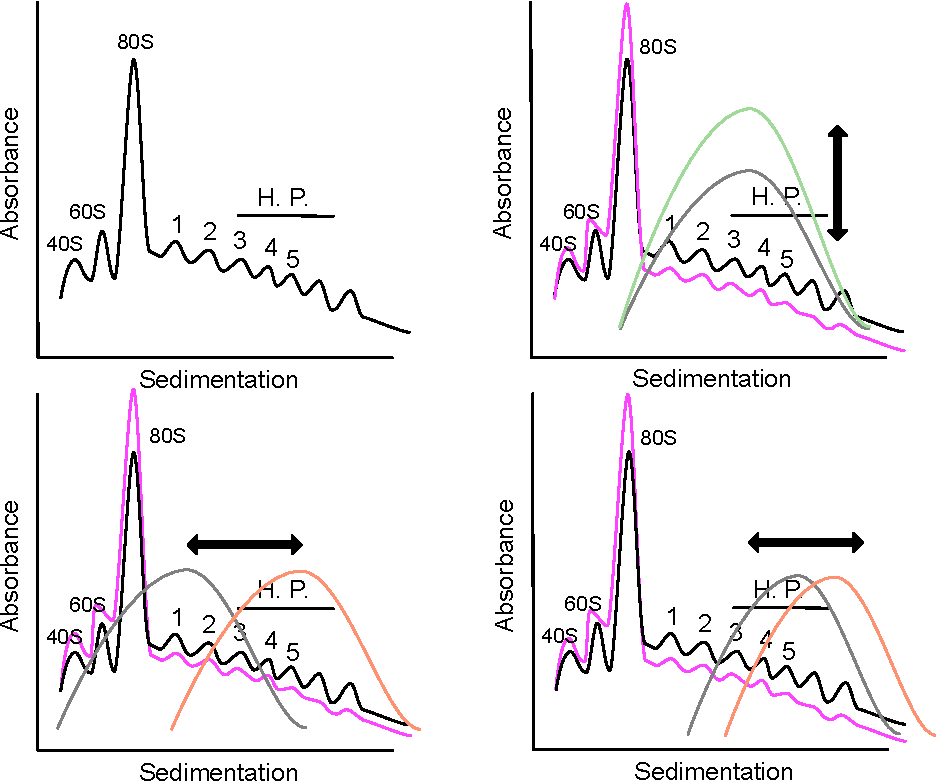
\includegraphics[width=0.9\linewidth]{./figures/polysome_shifts.pdf}
  \caption{Polysome profliles -  (top left) Schematic representation of a polysome profile using linear sucrose gradient fractionation. Indicated in the polysome profiles are the 40S, 60S ribosomal subunits as well as the 80S monosome. H.P. indicates heavy polysome fractions.Between conditions distribution changes for mRNA abundance (top right), translation (bottom left) and translation within high polysome fractions (bottom right) are illustrated. \label{fig:polysome}}
\end{wrapfigure}

The resulting gradient is fractionated and mRNAs with different number of bound ribosomes can be extracted and analyzed for changes in translational efficiency (Gandin et al., 2014). An illustration of a polysome profile with peaks for the 40S, 60S subunits and 80S ribosome can be seen in (\textbf{Fig \ref{fig:polysome} top left}). Subsequent peaks along the frations indicate the mRNAs with 1 or more bound ribosome. mRNAs are typically normally distributed along the fractions, i.e.~a pool of the same mRNA will be associated with 1- n number of ribosomes. Changes in mRNA abundance will lead to an overall increase in the amount of isolated polysome-associated mRNA without a shift of the distribution along the fractions (\textbf{Fig \ref{fig:polysome} top right}). This means that the translation efficiency per mRNA remains unchanged. Changes in translational efficiency can be observed by shifts of polysome association for mRNAs from the light (inefficiently translated) towards the heavy (efficiently translated) polysome fractions or vice versa (\textbf{Fig \ref{fig:polysome} bottom left}). Shift within the heavy polysome fractions (i.e.~3 bound ribosome to 7 bound ribosome) can also occur (\textbf{Fig \ref{fig:polysome} bottom right}). These shift remain undetected in cases where the distribtion of polysome-associated mRNAs does not sufficiently shift across the fractions and is a limitation of polysome profiling. Quantification of mRNA levels within each fraction can be assessed using Northern blotting or reverse transcription quantitative polymerase chain reaction (RT-qPCR).
For transcriptome wide studies, pooling of efficiently translated mRNAs (mRNAs with \textgreater3 bound ribosomes) followed by quantification using either DNA-microarrays or RNA sequencing is common. Pooling of mRNAs as well as collection of multiple fractions makes polysome profiling inconvenient when dealing with large samples sizes or experiments with low amounts of input RNA. Therefore, an optimized sucrose gradient was developed where most efficiently translated mRNAs are collected on a sucrose cushion and thereby can be isolated from one single fraction (Liang et al., 2018). This optimized gradient allows for application of polysome profiling in small tissue samples where RNA quantity is limiting and reduces labor intensity of the assay.
Polysome-associated mRNA levels are subject to changes in translation efficiency as well as factors contributing to cytosolic mRNA levels. Mechanisms such as transcription (i.e.~in the case of mRNA abundance) or mRNA stability can affect cytosolic mRNA levels which impacts the pool of mRNAs that can be associated to polysomes. Therefore, to identify bona fide changes in translation efficiency it is important to collect cytoplasmic mRNA levels in parallel to polysome-associated mRNA to correct for such mechanisms (e.g.~transcription or mRNA stability) during downstream analysis Oertlin et al. (2019).

\subsection{Ribosome profiling}

is a technique that enables sequencing of ribosome protected mRNA fragments (RPFs). In the assay ribosomes are immobilized on the mRNAs using, similar to polysome profiling, translation elongations inhibitors (e.g.~cyclohexamide) Ingolia (2016). One limitation with the use of translation elongation inhibitors is the distortion of ribosome distributions especially at translation initiation sites. These introduced artefacts need to be accounted for in the downstream analysis when assessing ribosome position along the mRNA. Following the translation elongation inhibitor treatment, cells ought to be immediately flash frozen using liquid nitrogen. Alternatively, using only flash freezing has been seen as a robust approach in a wide range of diverse organisms (Brar \& Weissman, 2015). Generation of RPFs is achieved by RNAse treatment breaking the links of RNA between ribosomes leaving single ribosomes with a \textasciitilde28 nucleotide long RNA fragment within each ribosome. RPFs are then isolated using ultra centrifugation through a sucrose cushion. Co-migration of RNA fragments such as structured non-coding RNAs or large ribonucleoprotein complexes within the sucrose gradient can be a cause of contamination and thereby can provide false readouts of translation. A polyacrylamide gel loaded with RPFs and a reference ladder is used to select RPFs of the right size. Typically, RPFs with lengths of 25 to 30 nucleotides are selected. The RPFs can then be pooled if sample specific barcodes are used. After size selection a pre-adenylated DNA is ligated to the RPFs. This RNA-DNA construct is then used as template for reverse transcription. Through gel-based purification, full-length products of the reverse transcription are selected and circularized. Following circularization, a double stranded DNA library is constructed and PCR amplified. This library is suitable for quantification using RNAseq. In parallel to RPF selection, randomly fragmented total mRNA of the same size is also retrieved. This is achieved by extraction of total mRNA from cell lysate followed by purification via recovery of polyadenylated messages or removal of ribosomal RNA. Fragmentation of total RNA is done using an alkaline fragmentation buffer Brar \& Weissman (2015).

\subsection{Comparing ribosome and polysome profiling}

Albeit both methods generate count data after quantification with RNAsequencing, there are some key aspects that differ between the techniques. Polysome profiling separates efficiently translated mRNAs from non- efficiently translated mRNAs along a sucrose thereby creating an mRNA based perspective for analyzing changes in translational efficiencies. In contrast, ribosome profiling determines translational efficiencies by counting the number of RPFs of both efficiently and non-efficiently translated mRNAs. Changes in translational efficiencies, e.g.~shifts between the polysomal fractions, can be dramatic (I.e. near complete dissociation of ribosomes from an mRNA) or subtle (shifts from 2 to 4 ribosomes) (Livingstone et al., 2015). Ribosome profiling has been shown to be biased towards identification of dramatic shifts of associated ribosomes to mRNAs, whereas subtle shifts are masked which can lead to false biological conclusions. Polysome profiling is affected by this to a much lesser extent, thereby more robust in identifying such changes (Masvidal, Hulea, Furic, Topisirovic, \& Larsson, 2017). RPFs in ribosome profiling provide exact nucleotide positions occupied by ribosomes thereby offering single nucleotide resolution. Polysome profiling cannot reveal ribosome locations along the mRNA. However, polysome profiling allows access to full-length mRNAs that includes the UTRs. The single nucleotide resolution of ribosome profiling is necessary in contexts studying local translation events such as ribosomal frame shifts (Rato, Amirova, Bates, Stansfield, \& Wallace, 2011) or uORF translation (Andreev et al., 2015). Higher sensitivity in detecting changes in translational efficiencies on a global scale makes polysome profiling more suitable for transcriptome-wide studies (Gandin et al., 2016). Both methods have their strengths and weaknesses and therefore each method should be considered depending on the underlying biological question of each experiment.

\section{Algorithms for analysis of changes in translation efficiencies}

In polysome-profiling and ribosome profiling translated mRNAs (i.e.~polysome-associated mRNAs and RPFs) are separated in parallel from their total mRNA counterpart. Estimating translation efficiencies requires that changes in translated mRNA are corrected for changes in total mRNA to accurately identify the regulatory modes of gene expression (i.e.~translation, mRNA abundance and translational buffering)(Oertlin et al., 2019). Here we will discuss methods that analyse polysome-profiling and ribosome profiling data to estimate changes in translation efficiencies across 2 or more conditions and how these methods identify different regulatory modes of gene expression.

Initially analysis of transcriptome-wide translation studies used an approach called the translation efficiency (TE-score) that uses the following equation:
\[\varDelta TE = \frac{\frac{P_{c2}}{T_{c2}}} {\frac{P_{c1}}{T_{c1}}}\\\]

This score calculates the ratio of the ratios between polysome-associated mRNA levels (P) divided by total mRNA levels (T) within each condition (i.e.~C1 and C2). The TE- score approach has been shown to be prone to spurious correlations (Larsson, Sonenberg, \& Nadon, 2010). Spurious correlations arise due to that the ratio of polysome-associated mRNA and total mRNA can systematically correlate with total mRNA levels which is not corrected for in this equation and leads to an elevated type-1 error.
\clearpage

\begin{wrapfigure}{o}{0.5\textwidth}
  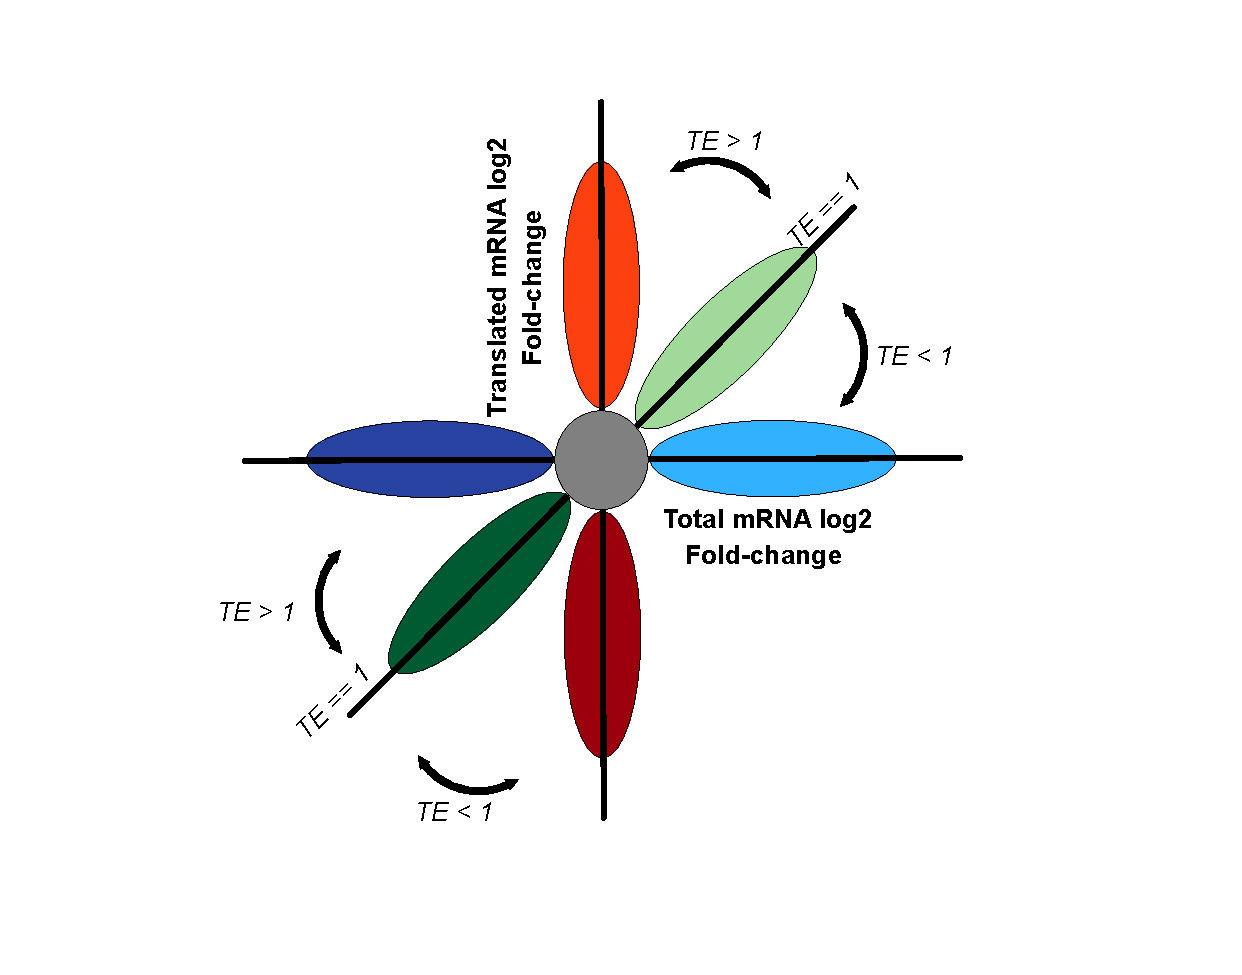
\includegraphics{./figures/geneModes_TE.pdf}
  \caption{TE scores for regulatory modes of gene expression -  Schematic representation of regulatory modes of translation efficiency in a fold-change scatter plot. Indicated in red are changes in translation efficiency altering protein levels, in green changes in mRNA abundance and in blue changes in translation efficiency leading to translational buffering/offsetting. The shifts for the translation efficiency (TE) score are indicated. \label{fig:TE}}
\end{wrapfigure}

\textbf{Figure \ref{fig:TE}} gives an overview of the relationship between a change in TE) and each regulatory mode of gene expression. Changes in mRNA abundance will lead to a \(\varDelta\)TE close to 0 in log space (i.e.~no change) as total mRNA and translated mRNA change with a similar magnitude. However, in the case of both translation and translational buffering, terms in the TE-score equation change leading to a \(\varDelta\)TE (TE \textless{} 0 or TE \textgreater{} 0) and thereby identification of both changes in translation and translational buffering simultaneously. Therefore, the TE-score method fails to differentiate between changes in translation and translational buffering which can have drastic consequences for the biological interpretation of the results (Oertlin et al., 2019).

The TE-score approach was challenged by the Analysis of Translation Activity (anota) algorithm which was developed for DNA-microarray data (Larsson, Sonenberg, \& Nadon, 2011). anota combines analysis of partial variance (APV)(Schleifer, Eckholdt, Cohen, \& Keller, 1993) with a random variance model (RVM)(Wright \& Simon, 2003). RVM estimates gene variance using shared informatio across all genes to increase power for detection of differential expression(Wright \& Simon, 2003). anota uses a two-step process that firstly assesses the model assumptions for (i) absence of highly influential data points, (ii) common slopes of sample classes, (iii) homoscedasticity of residuals and (iv) normal distribution of per gene residuals. In the second step then performs analysis of changes in translational activity using the following model:

\[log(y_{gi}) = \beta_g^{RNA}\ X_i^{RNA}+ \beta_g^{cond}\ X_i^{cond} + \varepsilon_{gi}\]

here \(\beta_g^{RNA}\) is the log2 fold change for total mRNA \(gth\) gene \(ith\) sample of model matrix \(X\); \(\beta_g^{cond}\) represent the log2 fold change for treatment classes and \(\varepsilon_{gi}\) denotes the residual error.

\begin{wrapfigure}{o}{0.5\textwidth}
  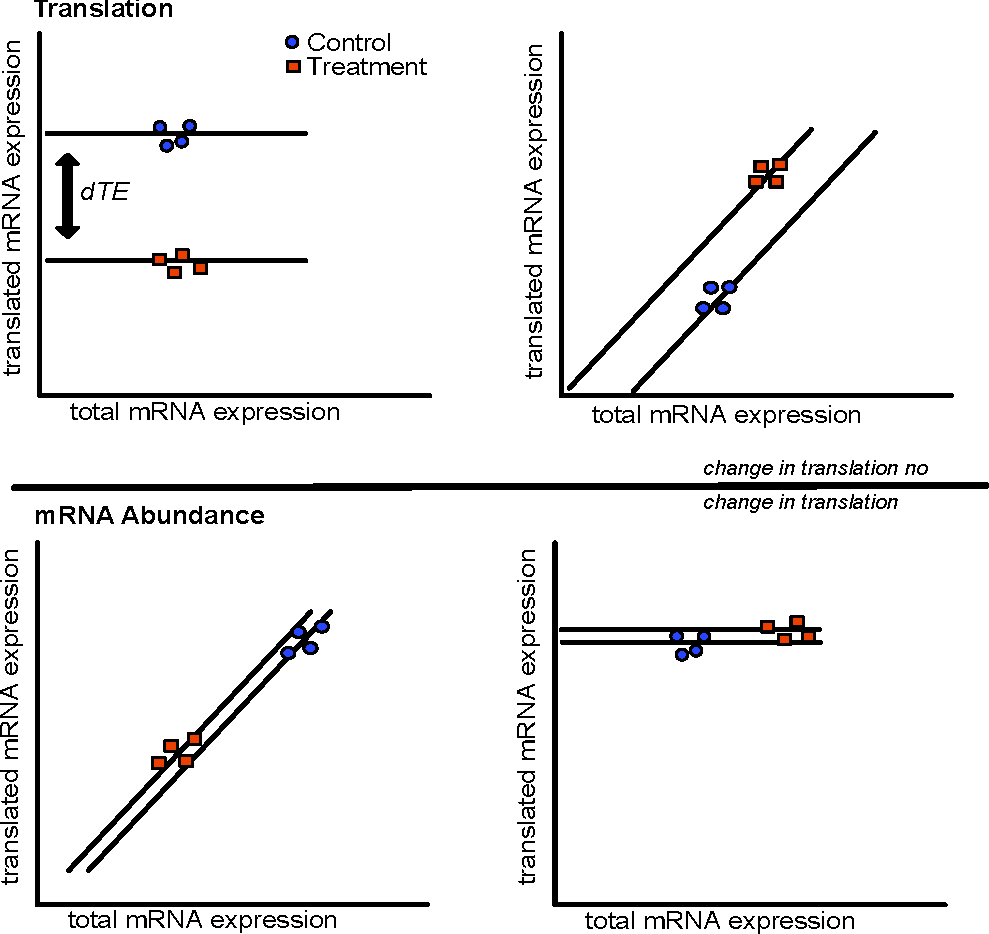
\includegraphics{./figures/geneModes_anota_Larsson.pdf}
  \caption{anota gene models - Schematic representation of the anota analysis models. Translation mRNA expression is set out against total mRNA expression for each biological replicate and treatment condition. Top left shows the model of a gene that is differentially translated (i.e. change in translated but not total mRNA). The difference in the slope intercepts are used to estimate changes in translation efficiencies between conditions i.e. dTE. Other gene models are shown; change in translation efficiency with varying total mRNA levels (top right); change in mRNA abundance (bottom left) and translational buffering (bottom right).
  \label{fig:anota}}
\end{wrapfigure}

Within anota a common slope for the treatment classes that describes the translated mRNA to total mRNA relationship is calculated. The difference between the slope intercepts is then interpreted as the \(\varDelta\) TE. A simplified view of this model can be seen in (\textbf{Figure \ref{fig:anota} top left}). Here expression for translated mRNA and total mRNA are modeled over two sample classes with each 4 replicates. Furthermore, changes in translation efficiencies can also be observed when translated mRNAs shift to a larger extent than the total mRNA levels (\textbf{Figure \ref{fig:anota} top right}). Identification of genes in this categorie can be a challenge, especially in highyl variable data set, as they resemble mRNA abundance genes (\textbf{Figure \ref{fig:anota} bottom left}). Nevertheless, Using the linear regression analysis anota accurately corrects changes in translated mRNA as can be seen in (\textbf{Figure \ref{fig:anota} bottom right}) where a change in total mRNA but not translated mRNA levels is observed. For this gene the difference in slope intercepts is small and will not be identified as difference in translation as would be the case in the TE-score approach. anota was developed at a time where translational buffering was uncommonly seen in data sets. Naturally, the methods lacks a setting to analyse translational buffering. This was addressed in anota's successor, anota2seq, and will be discussed in \textbf{Study 1}.

Advances in experimental methods warrant for appropriate statistical methods to analyse data resulting from them. DNA- microarray was the dominant platform to assess genome-wide changes before the advent of RNA sequencing. In DNA- microarray RNA hybridizes probes on a chip and generate a signal of which the measured intensity is an indicator of expression, whereas in RNA sequencing reads from RNAs are counted. Intensity data from DNA microarray can be normalised and transformed (i.e.~log transformation) to fulfill the requirements for application of linear models, whereas RNA sequencing harbours additional characteristics that need to be accounted for. Therefore, algorithms developed for analysis of DNA- microarray are not directly applicable to RNA sequencing data as is the case for the anota algorithm.

RNA sequencing data shows variance that is greater than the mean which is commonly referred to as overdispersion. Count data from RNA sequencing have been initially approached using Poisson distributions which assumes that the variance is equal to the mean(Lu, Tomfohr, \& Kepler, 2005). Now established RNA sequencing analysis frameworks such as edgeR and DESeq2 use negative binomial distributions in combination with generalized linear models (GLMs) Love, Huber, \& Anders (2014). The negative binomial distribution uses a dispersion parameter to account for overdispersion (McCarthy, Chen, \& Smyth, 2012). While analysis principles of DESeq2 and edgeR are similar they differ in their normalisation method, dispersion estimation and information sharing across genes. In a simple differential expression analysis between two conditions with one RNA type the GLM model would be as in the following equation:

\[log(y_{gi}) = \beta_g^{cond}\ X_i^{cond} + \varepsilon_{gi}\]

here \(\beta_g^{cond}\ X_i^{cond}\) represent the condition (i.e.~control and treatment) log2 fold change for the \(gth\) gene \(ith\) sample of the model matrix X and \(\varepsilon_{gi}\) denotes the residual error. When analysing changes in translation effiencies additional parameter for RNA type (i.e.~total mRNA or translated mRNA) and the interaction between the RNA type and condition are added so that:

\[log(y_{gi}) = \beta_g^{RNA}\ X_i^{RNA}+ \beta_g^{cond}\ X_i^{cond} + \beta_g^{RNA:cond}\ X_i^{interaction} + \varepsilon_gi\]

In this model the interaction term is interpreted as the change in translation effiencies (Chothani et al., 2019). Other methods (i.e.~Ribodiff(Zhong et al., 2017), Riborex(W. Li, Wang, Uren, Penalva, \& Smith, 2017) and deltaTE (Chothani et al., 2019)) borrow this analysis principle of an GLM with an interaction term by often applying this exact model. A noteable difference is that Ribodiff allows dispersion estimation for translated mRNA and total mRNA separetly as variance differences between the RNA types can be expected due to varying experimental protocols Liang et al. (2018). While the flexibility of GLMs allows for complex study designs involving 2 or more treatment conditions, Riborex and Ribodiff limit the study design to only two conditions. DeltaTE gives their users full flexibility of the DESeq2 GLM model. Xtail is a method developed for ribosome profiling that makes use of DESeq2 for RNAseq count normalisation (Xiao, Zou, Liu, \& Yang, 2016). Their assessment of differences in translation efficiencies relies on probability matrices for the ratio of translated mRNA over total mRNA within condition and a between condition ratio of these ratios. Babel was the first algorithm designed solely for analysis of differential translation and uses an error-in-varaibles regression analysis (Olshen et al., 2013). The error-in- variables regression allows accounting for variable total mRNA levels when assessing changes in translation. Although these methods have distinct approaches to identify changes in translation efficiencies, their principle of analysis is similar to comparing a ratio of ratios. Therefore these methods suffer from similar issues as the TE-score which will be discussed in \textbf{Study 1}.

\section{mRNA translation in cancer}

\chapter{Aims of this thesis}

The aims of this thesis are to expand current methodologies for analysis of translation efficiency data and explore the regulation of gene expression in cancer.

In \textbf{Study I} we adapted an algorithm for ANalysis Of Translation Activity data (anota) so that it could be applied to next generation sequencing data. Furthermore, we implemented the analysis of translational buffering a recently described regulatory mode of gene expression. The resulting algorithm was named anota2seq.

We then applied the anota2seq algorithm to investigate changes in translation efficiencies in two cancer models:

In \textbf{Study II} we unravelled the effects of eIF4A, an RNA helicase, inhibition using a synthetic rocaglate CR-1-31-B (CR-31) in pancreatic ductal adenocarcinoma.

In \textbf{Study III} we explored the effects of insulin on gene expression in multiple cell lines.

\chapter{Results and discussion}

\chapter{Conclusions}

\hypertarget{acknowledgments}{%
\chapter*{Acknowledgments}\label{acknowledgments}}
\addcontentsline{toc}{chapter}{Acknowledgments}

Christina is awesome.

I am sorry for all the other people of this page but no one else helped me more than my 8 paws of awesomeness Felix and Dexter. These little litter shitters have been an extreme joy to be around and kept me sane during the insanity that is writing a thesis. \textbf{Meow}

\hypertarget{references}{%
\chapter*{References}\label{references}}
\addcontentsline{toc}{chapter}{References}

\hypertarget{refs}{}
\begin{CSLReferences}{1}{0}
\leavevmode\hypertarget{ref-Andreev2015}{}%
Andreev, D. E., O'Connor, P. B., Fahey, C., Kenny, E. M., Terenin, I. M., Dmitriev, S. E., \ldots{} Baranov, P. V. (2015). Translation of 5{\({'}\)} leaders is pervasive in genes resistant to {eIF2} repression. \emph{eLife}, \emph{4}, e03971. \url{https://doi.org/10.7554/eLife.03971}

\leavevmode\hypertarget{ref-Artieri2014}{}%
Artieri, C. G., \& Fraser, H. B. (2014). Evolution at two levels of gene expression in yeast. \emph{Genome Research}, \emph{24}(3), 411--421. \url{https://doi.org/10.1101/gr.165522.113}

\leavevmode\hypertarget{ref-Avni1997}{}%
Avni, D., Biberman, Y., \& Meyuhas, O. (1997). The 5{\({'}\)} {Terminal Oligopyrimidine Tract Confers Translational Control} on {Top Mrnas} in a {Cell Type}-and {Sequence Context}-{Dependent Manner}. \emph{Nucleic Acids Research}, \emph{25}(5), 995--1001. \url{https://doi.org/10.1093/nar/25.5.995}

\leavevmode\hypertarget{ref-Brar2015}{}%
Brar, G. A., \& Weissman, J. S. (2015). Ribosome profiling reveals the what, when, where and how of protein synthesis. \emph{Nature Reviews. Molecular Cell Biology}, \emph{16}(11), 651--664. \url{https://doi.org/10.1038/nrm4069}

\leavevmode\hypertarget{ref-Buttgereit1995}{}%
Buttgereit, F., \& Brand, M. D. (1995). A hierarchy of {ATP}-consuming processes in mammalian cells. \emph{The Biochemical Journal}, \emph{312 ( Pt 1)}(Pt 1), 163--7. \url{https://doi.org/10.1042/bj3120163}

\leavevmode\hypertarget{ref-Carayol2008}{}%
Carayol, N., Katsoulidis, E., Sassano, A., Altman, J. K., Druker, B. J., \& Platanias, L. C. (2008). Suppression of programmed cell death 4 ({PDCD4}) protein expression by {BCR}-{ABL}-regulated engagement of the {mTOR}/P70 {S6} kinase pathway. \emph{The Journal of Biological Chemistry}, \emph{283}(13), 8601--10. \url{https://doi.org/10.1074/jbc.M707934200}

\leavevmode\hypertarget{ref-Cenik2015}{}%
Cenik, C., Cenik, E. S., Byeon, G. W., Grubert, F., Candille, S. I., Spacek, D., \ldots{} Snyder, M. P. (2015). Integrative analysis of {RNA}, translation, and protein levels reveals distinct regulatory variation across humans. \emph{Genome Research}, \emph{25}(11), 1610--1621. \url{https://doi.org/10.1101/gr.193342.115}

\leavevmode\hypertarget{ref-Cheng2013}{}%
Cheng, S., \& Gallie, D. R. (2013). Eukaryotic initiation factor {4B} and the poly({A})-binding protein bind {eIF4G} competitively. \emph{Translation (Austin, Tex.)}, \emph{1}(1), e24038. \url{https://doi.org/10.4161/trla.24038}

\leavevmode\hypertarget{ref-Chothani2019}{}%
Chothani, S., Adami, E., Ouyang, J. F., Viswanathan, S., Hubner, N., Cook, S. A., \ldots{} Rackham, O. J. L. (2019). {deltaTE}: {Detection} of {Translationally Regulated Genes} by {Integrative Analysis} of {Ribo}-seq and {RNA}-seq {Data}. \emph{Current Protocols in Molecular Biology}, \emph{129}(1), e108. \url{https://doi.org/10.1002/cpmb.108}

\leavevmode\hypertarget{ref-Darnell2011}{}%
Darnell, J. C., Van Driesche, S. J., Zhang, C., Hung, K. Y. S., Mele, A., Fraser, C. E., \ldots{} Darnell, R. B. (2011). {FMRP Stalls Ribosomal Translocation} on {mRNAs Linked} to {Synaptic Function} and {Autism}. \emph{Cell}, \emph{146}(2), 247--261. \url{https://doi.org/10.1016/j.cell.2011.06.013}

\leavevmode\hypertarget{ref-delaParra2018}{}%
de la Parra, C., Ernlund, A., Alard, A., Ruggles, K., Ueberheide, B., \& Schneider, R. J. (2018). A widespread alternate form of cap-dependent {mRNA} translation initiation. \emph{Nature Communications}, \emph{9}(1), 3068. \url{https://doi.org/10.1038/s41467-018-05539-0}

\leavevmode\hypertarget{ref-Deragon2015}{}%
Deragon, J.-M., \& Bousquet-Antonelli, C. (2015). The role of {LARP1} in translation and beyond. \emph{Wiley Interdisciplinary Reviews. RNA}, \emph{6}(4), 399--417. \url{https://doi.org/10.1002/wrna.1282}

\leavevmode\hypertarget{ref-Dever2012}{}%
Dever, T. E., \& Green, R. (2012). The elongation, termination, and recycling phases of translation in eukaryotes. \emph{Cold Spring Harbor Perspectives in Biology}, \emph{4}(7), 1--16. \url{https://doi.org/10.1101/cshperspect.a013706}

\leavevmode\hypertarget{ref-Fonseca2014}{}%
Fonseca, Bruno D., Smith, E. M., Yelle, N., Alain, T., Bushell, M., \& Pause, A. (2014). The ever-evolving role of {mTOR} in translation. \emph{Seminars in Cell \& Developmental Biology}, \emph{36}, 102--112. \url{https://doi.org/10.1016/j.semcdb.2014.09.014}

\leavevmode\hypertarget{ref-Fonseca2015}{}%
Fonseca, Bruno D., Zakaria, C., Jia, J.-J., Graber, T. E., Svitkin, Y., Tahmasebi, S., \ldots{} Damgaard, C. K. (2015). La-related {Protein} 1 ({LARP1}) {Represses Terminal Oligopyrimidine} ({TOP}) {mRNA Translation Downstream} of {mTOR Complex} 1 ({mTORC1}). \emph{The Journal of Biological Chemistry}, \emph{290}(26), 15996--6020. \url{https://doi.org/10.1074/jbc.M114.621730}

\leavevmode\hypertarget{ref-Gandin2016}{}%
Gandin, V., Masvidal, L., Cargnello, M., Gyenis, L., McLaughlan, S., Cai, Y., \ldots{} Topisirovic, I. (2016). {mTORC1} and {CK2} coordinate ternary and {eIF4F} complex assembly. \emph{Nature Communications}, \emph{7}(1), 11127. \url{https://doi.org/10.1038/ncomms11127}

\leavevmode\hypertarget{ref-Gandin2014}{}%
Gandin, V., Sikström, K., Alain, T., Morita, M., McLaughlan, S., Larsson, O., \& Topisirovic, I. (2014). Polysome fractionation and analysis of mammalian translatomes on a genome-wide scale. \emph{Journal of Visualized Experiments: JoVE}, (87). \url{https://doi.org/10.3791/51455}

\leavevmode\hypertarget{ref-Guan2017}{}%
Guan, B.-J., van Hoef, V., Jobava, R., Elroy-Stein, O., Valasek, L. S., Cargnello, M., \ldots{} Hatzoglou, M. (2017). A {Unique ISR Program Determines Cellular Responses} to {Chronic Stress}. \emph{Molecular Cell}, \emph{68}(5), 885--900.e6. \url{https://doi.org/10.1016/j.molcel.2017.11.007}

\leavevmode\hypertarget{ref-Guzeloglu-Kayisli2008}{}%
Guzeloglu-Kayisli, O., Pauli, S., Demir, H., Lalioti, M. D., Sakkas, D., \& Seli, E. (2008). Identification and characterization of human embryonic poly({A}) binding protein ({EPAB}). \emph{Molecular Human Reproduction}, \emph{14}(10), 581--588. \url{https://doi.org/10.1093/molehr/gan047}

\leavevmode\hypertarget{ref-Haimov2015}{}%
Haimov, O., Sinvani, H., \& Dikstein, R. (2015). Cap-dependent, scanning-free translation initiation mechanisms. \emph{Biochimica Et Biophysica Acta}, \emph{1849}(11), 1313--1318. \url{https://doi.org/10.1016/j.bbagrm.2015.09.006}

\leavevmode\hypertarget{ref-Hamilton2006}{}%
Hamilton, T. L., Stoneley, M., Spriggs, K. A., \& Bushell, M. (2006). {TOPs} and their regulation. \emph{Biochemical Society Transactions}, \emph{34}(1), 12--16. \url{https://doi.org/10.1042/BST0340012}

\leavevmode\hypertarget{ref-Hay2004}{}%
Hay, N., \& Sonenberg, N. (2004). Upstream and downstream of {mTOR}. \emph{Genes \& Development}, \emph{18}(16), 1926--1945. \url{https://doi.org/10.1101/gad.1212704}

\leavevmode\hypertarget{ref-Hinnebusch2006}{}%
Hinnebusch, Alan G. (2006). {eIF3}: A versatile scaffold for translation initiation complexes. \emph{Trends in Biochemical Sciences}, \emph{31}(10), 553--562. \url{https://doi.org/10.1016/j.tibs.2006.08.005}

\leavevmode\hypertarget{ref-Hinnebusch2014}{}%
Hinnebusch, Alan G. (2014). The scanning mechanism of eukaryotic translation initiation. \emph{Annual Review of Biochemistry}, \emph{83}, 779--812. \url{https://doi.org/10.1146/annurev-biochem-060713-035802}

\leavevmode\hypertarget{ref-Hsieh2010}{}%
Hsieh, A. C., Costa, M., Zollo, O., Davis, C., Feldman, M. E., Testa, J. R., \ldots{} Ruggero, D. (2010). Genetic {Dissection} of the {Oncogenic mTOR Pathway Reveals Druggable Addiction} to {Translational Control} via {4EBP}-{eIF4E}. \emph{Cancer Cell}, \emph{17}(3), 249--261. \url{https://doi.org/10.1016/j.ccr.2010.01.021}

\leavevmode\hypertarget{ref-Hu2014}{}%
Hu, W., Yuan, B., \& Lodish, H. F. (2014). Cpeb4-mediated translational regulatory circuitry controls terminal erythroid differentiation. \emph{Developmental Cell}, \emph{30}(6), 660--672. \url{https://doi.org/10.1016/j.devcel.2014.07.008}

\leavevmode\hypertarget{ref-Ingolia2010}{}%
Ingolia, N. T. (2010). Genome-wide translational profiling by ribosome footprinting. \emph{Methods in Enzymology}, \emph{470}, 119--142. \url{https://doi.org/10.1016/S0076-6879(10)70006-9}

\leavevmode\hypertarget{ref-Ingolia2016}{}%
Ingolia, N. T. (2016). Ribosome {Footprint Profiling} of {Translation} throughout the {Genome}. \emph{Cell}, \emph{165}(1), 22--33. \url{https://doi.org/10.1016/j.cell.2016.02.066}

\leavevmode\hypertarget{ref-Ivanov2016}{}%
Ivanov, A., Mikhailova, T., Eliseev, B., Yeramala, L., Sokolova, E., Susorov, D., \ldots{} Alkalaeva, E. (2016). {PABP} enhances release factor recruitment and stop codon recognition during translation termination. \emph{Nucleic Acids Research}, \emph{44}(16), 7766--7776. \url{https://doi.org/10.1093/nar/gkw635}

\leavevmode\hypertarget{ref-Jackson1991}{}%
Jackson, R. J. (1991). The {ATP} requirement for initiation of eukaryotic translation varies according to the {mRNA} species. \emph{European Journal of Biochemistry}, \emph{200}(2), 285--294. \url{https://doi.org/10.1111/j.1432-1033.1991.tb16184.x}

\leavevmode\hypertarget{ref-Jia2021}{}%
Jia, J.-J., Lahr, R. M., Solgaard, M. T., Moraes, B. J., Pointet, R., Yang, A.-D., \ldots{} Fonseca, B. D. (2021). {mTORC1} promotes {TOP mRNA} translation through site-specific phosphorylation of {LARP1}. \emph{Nucleic Acids Research}. \url{https://doi.org/10.1093/nar/gkaa1239}

\leavevmode\hypertarget{ref-Kapur2017}{}%
Kapur, M., Monaghan, C. E., \& Ackerman, S. L. (2017). Regulation of {mRNA Translation} in {Neurons}-{A Matter} of {Life} and {Death}. \emph{Neuron}, \emph{96}(3), 616--637. \url{https://doi.org/10.1016/j.neuron.2017.09.057}

\leavevmode\hypertarget{ref-Komar2005}{}%
Komar, A. A., \& Hatzoglou, M. (2005). Internal ribosome entry sites in cellular {mRNAs}: Mystery of their existence. \emph{The Journal of Biological Chemistry}, \emph{280}(25), 23425--23428. \url{https://doi.org/10.1074/jbc.R400041200}

\leavevmode\hypertarget{ref-Lalanne2018}{}%
Lalanne, J.-B., Taggart, J. C., Guo, M. S., Herzel, L., Schieler, A., \& Li, G.-W. (2018). Evolutionary {Convergence} of {Pathway}-{Specific Enzyme Expression Stoichiometry}. \emph{Cell}, \emph{173}(3), 749--761.e38. \url{https://doi.org/10.1016/j.cell.2018.03.007}

\leavevmode\hypertarget{ref-Laplante2012}{}%
Laplante, M., \& Sabatini, D. M. (2012). {mTOR Signaling}. \emph{Cold Spring Harbor Perspectives in Biology}, \emph{4}(2), a011593. \url{https://doi.org/10.1101/cshperspect.a011593}

\leavevmode\hypertarget{ref-Larsson2010}{}%
Larsson, O., Sonenberg, N., \& Nadon, R. (2010). Identification of differential translation in genome wide studies. \emph{Proceedings of the National Academy of Sciences}, \emph{107}(50), 21487--21492. \url{https://doi.org/10.1073/pnas.1006821107}

\leavevmode\hypertarget{ref-Larsson2011}{}%
Larsson, O., Sonenberg, N., \& Nadon, R. (2011). Anota: {Analysis} of differential translation in genome-wide studies. \emph{Bioinformatics (Oxford, England)}, \emph{27}(10), 1440--1441. \url{https://doi.org/10.1093/bioinformatics/btr146}

\leavevmode\hypertarget{ref-Lee2015}{}%
Lee, A. S. Y., Kranzusch, P. J., \& Cate, J. H. D. (2015). {eIF3} targets cell-proliferation messenger {RNAs} for translational activation or repression. \emph{Nature}, \emph{522}(7554), 111--114. \url{https://doi.org/10.1038/nature14267}

\leavevmode\hypertarget{ref-Leibovitch2018}{}%
Leibovitch, M., \& Topisirovic, I. (2018). Dysregulation of {mRNA} translation and energy metabolism in cancer. \emph{Advances in Biological Regulation}, \emph{67}, 30--39. \url{https://doi.org/10.1016/j.jbior.2017.11.001}

\leavevmode\hypertarget{ref-Li2014}{}%
Li, G.-W., Burkhardt, D., Gross, C., \& Weissman, J. S. (2014). Quantifying absolute protein synthesis rates reveals principles underlying allocation of cellular resources. \emph{Cell}, \emph{157}(3), 624--635. \url{https://doi.org/10.1016/j.cell.2014.02.033}

\leavevmode\hypertarget{ref-Li2017}{}%
Li, W., Wang, W., Uren, P. J., Penalva, L. O. F., \& Smith, A. D. (2017). Riborex: Fast and flexible identification of differential translation from {Ribo}-seq data. \emph{Bioinformatics (Oxford, England)}, \emph{33}(11), 1735--1737. \url{https://doi.org/10.1093/bioinformatics/btx047}

\leavevmode\hypertarget{ref-Liang2018}{}%
Liang, S., Bellato, H. M., Lorent, J., Lupinacci, F. C. S., Oertlin, C., van Hoef, V., \ldots{} Larsson, O. (2018). Polysome-profiling in small tissue samples. \emph{Nucleic Acids Research}, \emph{46}(1), e3. \url{https://doi.org/10.1093/nar/gkx940}

\leavevmode\hypertarget{ref-Livingstone2015}{}%
Livingstone, M., Sikström, K., Robert, P. A., Uzé, G., Larsson, O., \& Pellegrini, S. (2015). Assessment of {mTOR}-{Dependent Translational Regulation} of {Interferon Stimulated Genes}. \emph{PLOS ONE}, \emph{10}(7), e0133482. \url{https://doi.org/10.1371/journal.pone.0133482}

\leavevmode\hypertarget{ref-Lorent2019}{}%
Lorent, J., Kusnadi, E. P., van Hoef, V., Rebello, R. J., Leibovitch, M., Ristau, J., \ldots{} Furic, L. (2019). Translational offsetting as a mode of estrogen receptor {\(\alpha\)}-dependent regulation of gene~expression. \emph{The EMBO Journal}, \emph{38}(23), e101323. \url{https://doi.org/10.15252/embj.2018101323}

\leavevmode\hypertarget{ref-Love2014}{}%
Love, M. I., Huber, W., \& Anders, S. (2014). Moderated estimation of fold change and dispersion for {RNA}-seq data with {DESeq2}. \emph{Genome Biology}, \emph{15}(12), 550. \url{https://doi.org/10.1186/s13059-014-0550-8}

\leavevmode\hypertarget{ref-Lu2005}{}%
Lu, J., Tomfohr, J. K., \& Kepler, T. B. (2005). Identifying differential expression in multiple {SAGE} libraries: An overdispersed log-linear model approach. \emph{BMC Bioinformatics}, \emph{6}(1), 165. \url{https://doi.org/10.1186/1471-2105-6-165}

\leavevmode\hypertarget{ref-Magnuson2012}{}%
Magnuson, B., Ekim, B., \& Fingar, D. C. (2012). Regulation and function of ribosomal protein {S6} kinase ({S6K}) within {mTOR} signalling networks. \emph{Biochemical Journal}, \emph{441}(1), 1--21. \url{https://doi.org/10.1042/BJ20110892}

\leavevmode\hypertarget{ref-Masvidal2017}{}%
Masvidal, L., Hulea, L., Furic, L., Topisirovic, I., \& Larsson, O. (2017). {mTOR}-sensitive translation: {Cleared} fog reveals more trees. \emph{RNA Biology}, \emph{14}(10), 1299--1305. \url{https://doi.org/10.1080/15476286.2017.1290041}

\leavevmode\hypertarget{ref-Matoulkova2012}{}%
Matoulkova, E., Michalova, E., Vojtesek, B., \& Hrstka, R. (2012). The role of the 3'~untranslated region in post-transcriptional regulation of protein expression in mammalian cells. \emph{RNA Biology}, \emph{9}(5), 563--576. \url{https://doi.org/10.4161/rna.20231}

\leavevmode\hypertarget{ref-McCarthy2012}{}%
McCarthy, D. J., Chen, Y., \& Smyth, G. K. (2012). Differential expression analysis of multifactor {RNA}-{Seq} experiments with respect to biological variation. \emph{Nucleic Acids Research}, \emph{40}(10), 4288--4297. \url{https://doi.org/10.1093/nar/gks042}

\leavevmode\hypertarget{ref-McManus2014}{}%
McManus, C. J., May, G. E., Spealman, P., \& Shteyman, A. (2014). Ribosome profiling reveals post-transcriptional buffering of divergent gene expression in yeast. \emph{Genome Research}, \emph{24}(3), 422--430. \url{https://doi.org/10.1101/gr.164996.113}

\leavevmode\hypertarget{ref-Mendez2001}{}%
Mendez, R., \& Richter, J. D. (2001). Translational control by {CPEB}: A means to the end. \emph{Nature Reviews. Molecular Cell Biology}, \emph{2}(7), 521--529. \url{https://doi.org/10.1038/35080081}

\leavevmode\hypertarget{ref-Meyer2015}{}%
Meyer, K. D., Patil, D. P., Zhou, J., Zinoviev, A., Skabkin, M. A., Elemento, O., \ldots{} Jaffrey, S. R. (2015). 5' {UTR} m(6){A Promotes Cap}-{Independent Translation}. \emph{Cell}, \emph{163}(4), 999--1010. \url{https://doi.org/10.1016/j.cell.2015.10.012}

\leavevmode\hypertarget{ref-Moore2018}{}%
Moore, K. S., \& von Lindern, M. (2018). {RNA Binding Proteins} and {Regulation} of {mRNA Translation} in {Erythropoiesis}. \emph{Frontiers in Physiology}, \emph{9}, 910. \url{https://doi.org/10.3389/fphys.2018.00910}

\leavevmode\hypertarget{ref-Munroe1990}{}%
Munroe, D., \& Jacobson, A. (1990). {mRNA} poly({A}) tail, a 3' enhancer of translational initiation. \emph{Molecular and Cellular Biology}, \emph{10}(7), 3441--3455. \url{https://doi.org/10.1128/mcb.10.7.3441}

\leavevmode\hypertarget{ref-Oertlin2019}{}%
Oertlin, C., Lorent, J., Murie, C., Furic, L., Topisirovic, I., \& Larsson, O. (2019). Generally applicable transcriptome-wide analysis of translation using Anota2seq. \emph{Nucleic Acids Research}, \emph{47}(12), e70--e70. \url{https://doi.org/10.1093/nar/gkz223}

\leavevmode\hypertarget{ref-Oh2010}{}%
Oh, W. J., Wu, C. -chih, Kim, S. J., Facchinetti, V., Julien, L.-A., Finlan, M., \ldots{} Jacinto, E. (2010). {mTORC2} can associate with ribosomes to promote cotranslational phosphorylation and stability of nascent {Akt} polypeptide. \emph{The EMBO Journal}, \emph{29}(23), 3939--3951. \url{https://doi.org/10.1038/emboj.2010.271}

\leavevmode\hypertarget{ref-Olshen2013}{}%
Olshen, A. B., Hsieh, A. C., Stumpf, C. R., Olshen, R. A., Ruggero, D., \& Taylor, B. S. (2013). Assessing gene-level translational control from ribosome profiling. \emph{Bioinformatics (Oxford, England)}, \emph{29}(23), 2995--3002. \url{https://doi.org/10.1093/bioinformatics/btt533}

\leavevmode\hypertarget{ref-Pakos-Zebrucka2016}{}%
Pakos-Zebrucka, K., Koryga, I., Mnich, K., Ljujic, M., Samali, A., \& Gorman, A. M. (2016). The integrated stress response. \emph{EMBO Reports}, \emph{17}(10), 1374--1395. \url{https://doi.org/10.15252/embr.201642195}

\leavevmode\hypertarget{ref-Paraskeva1999}{}%
Paraskeva, E., Gray, N. K., Schläger, B., Wehr, K., \& Hentze, M. W. (1999). Ribosomal {Pausing} and {Scanning Arrest} as {Mechanisms} of {Translational Regulation} from {Cap}-{Distal} {Iron}-{Responsive Elements}. \emph{Molecular and Cellular Biology}, \emph{19}(1), 807--816.

\leavevmode\hypertarget{ref-Pearce2007}{}%
Pearce, L. R., Huang, X., Boudeau, J., Paw\textbackslash lowski, R., Wullschleger, S., Deak, M., \ldots{} Alessi, D. R. (2007). Identification of {Protor} as a novel {Rictor}-binding component of {mTOR} complex-2. \emph{Biochemical Journal}, \emph{405}(3), 513--522. \url{https://doi.org/10.1042/BJ20070540}

\leavevmode\hypertarget{ref-Perl2017}{}%
Perl, K., Ushakov, K., Pozniak, Y., Yizhar-Barnea, O., Bhonker, Y., Shivatzki, S., \ldots{} Shamir, R. (2017). Reduced changes in protein compared to {mRNA} levels across non-proliferating tissues. \emph{BMC Genomics}, \emph{18}(1), 305. \url{https://doi.org/10.1186/s12864-017-3683-9}

\leavevmode\hypertarget{ref-Rato2011}{}%
Rato, C., Amirova, S. R., Bates, D. G., Stansfield, I., \& Wallace, H. M. (2011). Translational recoding as a feedback controller: Systems approaches reveal polyamine-specific effects on the antizyme ribosomal frameshift. \emph{Nucleic Acids Research}, \emph{39}(11), 4587--4597. \url{https://doi.org/10.1093/nar/gkq1349}

\leavevmode\hypertarget{ref-Richter2015}{}%
Richter, J. D., \& Coller, J. (2015). Pausing on {Polyribosomes}: {Make Way} for {Elongation} in {Translational Control}. \emph{Cell}, \emph{163}(2), 292--300. \url{https://doi.org/10.1016/j.cell.2015.09.041}

\leavevmode\hypertarget{ref-Robinson2010}{}%
Robinson, M. D., McCarthy, D. J., \& Smyth, G. K. (2010). {edgeR}: A {Bioconductor} package for differential expression analysis of digital gene expression data. \emph{Bioinformatics}, \emph{26}(1), 139. \url{https://doi.org/10.1093/bioinformatics/btp616}

\leavevmode\hypertarget{ref-Roux2012}{}%
Roux, P. P., \& Topisirovic, I. (2012). Regulation of {mRNA} translation by signaling pathways. \emph{Cold Spring Harbor Perspectives in Biology}, \emph{4}(11), a012252. \url{https://doi.org/10.1101/cshperspect.a012252}

\leavevmode\hypertarget{ref-Roux2018}{}%
Roux, P. P., \& Topisirovic, I. (2018). Signaling {Pathways Involved} in the {Regulation} of {mRNA Translation}. \emph{Molecular and Cellular Biology}, \emph{38}(12). \url{https://doi.org/10.1128/MCB.00070-18}

\leavevmode\hypertarget{ref-Saxton2017}{}%
Saxton, R. A., \& Sabatini, D. M. (2017). {mTOR Signaling} in {Growth}, {Metabolism}, and {Disease}. \emph{Cell}, \emph{168}(6), 960--976. \url{https://doi.org/10.1016/j.cell.2017.02.004}

\leavevmode\hypertarget{ref-Schepetilnikov2013}{}%
Schepetilnikov, M., Dimitrova, M., Mancera-Martínez, E., Geldreich, A., Keller, M., \& Ryabova, L. A. (2013). {TOR} and {S6K1} promote translation reinitiation of {uORF}-containing {mRNAs} via phosphorylation of {eIF3h}. \emph{The EMBO Journal}, \emph{32}(8), 1087--1102. \url{https://doi.org/10.1038/emboj.2013.61}

\leavevmode\hypertarget{ref-Schleifer1993}{}%
Schleifer, S. J., Eckholdt, H. M., Cohen, J., \& Keller, S. E. (1993). Analysis of partial variance ({APV}) as a statistical approach to control day to day variation in immune assays. \emph{Brain, Behavior, and Immunity}, \emph{7}(3), 243--252. \url{https://doi.org/10.1006/brbi.1993.1025}

\leavevmode\hypertarget{ref-Seli2005}{}%
Seli, E., Lalioti, M. D., Flaherty, S. M., Sakkas, D., Terzi, N., \& Steitz, J. A. (2005). An embryonic poly({A})-binding protein ({ePAB}) is expressed in mouse oocytes and early preimplantation embryos. \emph{Proceedings of the National Academy of Sciences}, \emph{102}(2), 367--372. \url{https://doi.org/10.1073/pnas.0408378102}

\leavevmode\hypertarget{ref-Sonenberg2009}{}%
Sonenberg, N., \& Hinnebusch, A. G. (2009). Regulation of {Translation Initiation} in {Eukaryotes}: {Mechanisms} and {Biological Targets}. \emph{Cell}, \emph{136}(4), 731. \url{https://doi.org/10.1016/j.cell.2009.01.042}

\leavevmode\hypertarget{ref-Taniuchi2016}{}%
Taniuchi, S., Miyake, M., Tsugawa, K., Oyadomari, M., \& Oyadomari, S. (2016). Integrated stress response of vertebrates is regulated by four {eIF2\(\alpha\)} kinases. \emph{Scientific Reports}, \emph{6}, 32886. \url{https://doi.org/10.1038/srep32886}

\leavevmode\hypertarget{ref-Tcherkezian2014}{}%
Tcherkezian, J., Cargnello, M., Romeo, Y., Huttlin, E. L., Lavoie, G., Gygi, S. P., \& Roux, P. P. (2014). Proteomic analysis of cap-dependent translation identifies {LARP1} as a key regulator of 5'{TOP mRNA} translation. \emph{Genes \& Development}, \emph{28}(4), 357--371. \url{https://doi.org/10.1101/gad.231407.113}

\leavevmode\hypertarget{ref-Thakor2017}{}%
Thakor, N., Smith, M. D., Roberts, L., Faye, M. D., Patel, H., Wieden, H.-J., \ldots{} Holcik, M. (2017). Cellular {mRNA} recruits the ribosome via {eIF3}-{PABP} bridge to initiate internal translation. \emph{RNA Biology}, \emph{14}(5), 553--567. \url{https://doi.org/10.1080/15476286.2015.1137419}

\leavevmode\hypertarget{ref-Udagawa2013}{}%
Udagawa, T., Farny, N. G., Jakovcevski, M., Kaphzan, H., Alarcon, J. M., Anilkumar, S., \ldots{} Richter, J. D. (2013). Genetic and acute {CPEB1} depletion ameliorate fragile {X} pathophysiology. \emph{Nature Medicine}, \emph{19}(11), 1473--1477. \url{https://doi.org/10.1038/nm.3353}

\leavevmode\hypertarget{ref-Wang2001}{}%
Wang, X., Li, W., Williams, M., Terada, N., Alessi, D. R., \& Proud, C. G. (2001). Regulation of elongation factor 2 kinase by P90({RSK1}) and P70 {S6} kinase. \emph{The EMBO Journal}, \emph{20}(16), 4370--9. \url{https://doi.org/10.1093/emboj/20.16.4370}

\leavevmode\hypertarget{ref-Wolfe2014}{}%
Wolfe, A. L., Singh, K., Zhong, Y., Drewe, P., Rajasekhar, V. K., Sanghvi, V. R., \ldots{} Wendel, H.-G. (2014). {RNA G}-quadruplexes cause {eIF4A}-dependent oncogene translation in cancer. \emph{Nature}, \emph{513}(7516), 65--70. \url{https://doi.org/10.1038/nature13485}

\leavevmode\hypertarget{ref-Wright2003}{}%
Wright, G. W., \& Simon, R. M. (2003). A random variance model for detection of differential gene expression in small microarray experiments. \emph{Bioinformatics (Oxford, England)}, \emph{19}(18), 2448--2455. \url{https://doi.org/10.1093/bioinformatics/btg345}

\leavevmode\hypertarget{ref-Wurth2015}{}%
Wurth, L., \& Gebauer, F. (2015). {RNA}-binding proteins, multifaceted translational regulators in cancer. \emph{Biochimica Et Biophysica Acta}, \emph{1849}(7), 881--6. \url{https://doi.org/10.1016/j.bbagrm.2014.10.001}

\leavevmode\hypertarget{ref-Xiao2016}{}%
Xiao, Z., Zou, Q., Liu, Y., \& Yang, X. (2016). Genome-wide assessment of differential translations with ribosome profiling data. \emph{Nature Communications}, \emph{7}(1), 11194. \url{https://doi.org/10.1038/ncomms11194}

\leavevmode\hypertarget{ref-Yamashita2008}{}%
Yamashita, R., Suzuki, Y., Takeuchi, N., Wakaguri, H., Ueda, T., Sugano, S., \& Nakai, K. (2008). Comprehensive detection of human terminal oligo-pyrimidine ({TOP}) genes and analysis of their characteristics. \emph{Nucleic Acids Research}, \emph{36}(11), 3707--3715. \url{https://doi.org/10.1093/nar/gkn248}

\leavevmode\hypertarget{ref-Yang2003}{}%
Yang, H.-S., Jansen, A. P., Komar, A. A., Zheng, X., Merrick, W. C., Costes, S., \ldots{} Colburn, N. H. (2003). The transformation suppressor {Pdcd4} is a novel eukaryotic translation initiation factor {4A} binding protein that inhibits translation. \emph{Molecular and Cellular Biology}, \emph{23}(1), 26--37. \url{https://doi.org/10.1128/mcb.23.1.26-37.2003}

\leavevmode\hypertarget{ref-Zhong2017}{}%
Zhong, Y., Karaletsos, T., Drewe, P., Sreedharan, V. T., Kuo, D., Singh, K., \ldots{} Rätsch, G. (2017). {RiboDiff}: Detecting changes of {mRNA} translation efficiency from ribosome footprints. \emph{Bioinformatics (Oxford, England)}, \emph{33}(1), 139--141. \url{https://doi.org/10.1093/bioinformatics/btw585}

\end{CSLReferences}

\end{document}
